% Локализация маловероятных регионов и т.п.
\subsection{Векторизация с помощью удаления маловероятных регионов из плоского цикла}\label{sec:text_4_loc_branch}

Наличие команд передачи управления по условию в теле плоского цикла является основной причиной потери производительности при проведении векторизации.
При наличии большого количества операторов управления (гнезда циклов, операторы if, switch, break, continue) оптимизирующий компилятор либо создает крайне неэффективный векторный код, либо вообще отказыватся от векторизации из-за слишком низкого теоретического ожидания ускорения \cite{Rybakov2018VecBranch}.
Зачастую не весь код в теле векторизуемого цикла одинакого вероятен в процессе исполнения.
В случае, если в теле присутствуют явно низковероятные регионы, то можно выполнить их вынос из цикла, а оставшийся после преобразования код в теле цикла может быть векторизован либо автоматически, либо с минимальными усилиями.

\subsubsection{Вынос маловероятного региона из плоского цикла}

Рассмотрим оптимизацию выноса маловероятного региона из цикла с помощью временного сохранения условия.
Пусть есть плоский цикл, записанный в виде, представленном на листинге~\ref{lst:text_4_vec_loc_branch_1}

\begin{lstlisting}[caption={Плоский цикл с маловероятным регионом.},label={lst:text_4_vec_loc_branch_1}]
for (int i = 0; i < w; ++i)
{
    block(i);
    
    if (cond(i))
    {
        block_true(i); // prob. ~100%
    }
    else
    {
        block_false(i); // prob. ~0%
    }
}
\end{lstlisting}

В плоском цикле с листинга~\ref{lst:text_4_vec_loc_branch_1} внутри его тела мы видим три блока с кодом.
Блок кода \texttt{block(i)} выполнятся безусловно в начале тела цикла.
А далее в зависимости от вычисленного условия \texttt{cond(i)} (условие зависит от номера итерации, иначе можно было бы выполнить статическое расщепление цикла по условию) выполняется либо блок кода \texttt{block\_true(i)} (с вероятностью, близкой к ста процентам), либо блок \texttt{block\_false(i)} (с вероятностью, близкой к нулю).
Будем считать, что блок \texttt{block(i)}, а также вероятный код, является простым по структуре и пригодным для векторизации, тогда как код из блока \texttt{block\_false(i)} должен выполняться редко, обрабатывает некоторые исключительные случаи и содержит крайне разветвленный и непригодный для векторизации контекст.
В исходном виде компилятор, как правило, не справляется с векторизацией данного цикла, поэтому для его автоматической векторизации можно использовать преобразование исходного кода, связанное с расщеплением данного цикла по условию.

Для выполнения расщепления по условию создадим вместо одного цикла три новых.
В первом цикле будем выполняться только блок \texttt{block(i)}, после которого все условия \texttt{cond(i)} записываются в локальный массив булевых значений (в маску).
Во втором цикле на каждой итерации при истинном значении элемента \texttt{TMP[i]} выполняется ветка код из блока \texttt{block\_true(i)}.
Запись \texttt{block\_true(i) ? TMP[i]} означает выполнение блока под предикатом.
Третий же цикл инкапсулирует в себе выполнение маловероятного кода при условии ложности соответствующих значений \texttt{TMP[i]}.

\begin{lstlisting}[caption={Расщепление плоского цикла с маловероятным регионом.},label={lst:text_4_vec_loc_branch_2}]
for (int i = 0; i < w; ++i)
{
    block(i);
    TMP[i] = cond(i);
}

for (int i = 0; i < w; ++i)
{
    block_true(i) ? TMP[i];
}

if (TMP != 0x0)
{
    for (int i = 0; i < w; ++i)
    {
        if (!TMP[i])
        {
            block_false(i);
        }
    }
}
\end{lstlisting}

В результате выполненных преобразований первый цикл из листинга~\ref{lst:text_4_vec_loc_branch_2} содержит только векторизуемый безусловный код, второй цикл также содержит векторизуемый код, но с использованием предиката, который при векторизации преобразуется в векторную маску, накладываемую на все операции этого цикла.
Третий код является маловероятным и его вообще не требуется оптимизировать (дополнительно перед его выполнением следует проверить маску на наличие в ней ложных элементов, что также в большинстве случаев избавит от необходимости выполнять все итерации цикла).
В результате схематично векторизованная версия всех трех циклов будет выглядеть так, как это представлено на листинге~\ref{lst:text_4_vec_loc_branch_3}.

\begin{lstlisting}[caption={Векторизованная версия расщепленного плоского цикла с маловероятным регионом.},label={lst:text_4_vec_loc_branch_3}]
BLOCK();
TMP = COND();
BLOCK_TRUE() ? TMP;

if (TMP != 0x0)
{
    for (int i = 0; i < w; ++i)
    {
        if (!TMP[i])
        {
            block_false(i);
        }
    }
}
\end{lstlisting}

Это преобразования следует использовать при уверенности, что условие \texttt{cond(i)} является вероятным.
При значении вероятности данного условия, близкой к 100\%, теоретическое ускорение от применения векторизации будет близко к ширине векторизации (при условии, что \texttt{block(i)} и \texttt{block\_true(i)}> векторизуются идеально).
Однако, если условие \texttt{cond(i)} не является вероятным, то выполнение такого преобразования приведет к деградации производительности.

\subsubsection{Эксперимент по применению выноса маловероятного региона для повышения эффективности векторизации}

В разделе~\ref{sec:text_1_geo_prim_line_eps_intersect} была описана задача нахождения пересечения прямой с окрестностью отрезка в пространстве.
Эта задача имеет практическое значение в авиации применительно к обеспечению безопасности полетов воздушных судов.
Во время полета летательный аппарат генерирует вихревой спутный след \cite{Aubakirov1999Wake}, который со временем эволюционирует и конечном итоге разрушается \cite{Vyshinsky2006Wake}.
Этот след может представлять опасность для других участников воздушного движения \cite{Babkin2008Wake}, особенно в зонах, содержащих большое число летательных аппаратов \cite{Burluzky2014Wake}.
Вихревой след может рассматриваться как совокупность окрестностей отдельных отрезков траектории движения.
Для определения конфликта требуется решить задачу наличия пересечения траектории движения собственного летательного аппарата (которая представлена полупрямой) с множеством окрестностей отрезков.
При этом наличие хотя бы одного пересечения является редкой исключительной ситуацией, требующей немедленной обработки.
Если рассматривать поставленную задачу в виде плоского цикла, то вероятной ветвью исполнения в нем будем анализ на наличие пересечения, а маловероятной -- находения самих точек пересечения и принятие решения об избежании конфликта \cite{Rybakov2017Flight,Rybakov2022VecGeom}.

Рассмотрим задачу пересечения траектории собственного летательного аппарата с окрестностью какого-либо отрезка движения другого летательного аппарата.
Решение этой задачи приведено в разделе~\ref{sec:text_1_geo_prim_line_eps_intersect}.

Рассмотрим неравенство \eqref{eqn:text_1_geo_prim_ineq_k2k1k0} и случай $k_2 < 0$.
Распишем это условие подробнее (см. \eqref{eqn:text_1_geo_prim_k2k1k0})
\begin{equation}
	k_2 = (\Delta \overline{C}, \overline{V})^2 + |\overline{V}|^2 \left( \Delta R^2 - |\Delta \overline{C}|^2 \right)
\end{equation}

Раскрыв скалярное произведение векторов и выполнив необходимые преобразования, получим следующее условие на угол между тректорией движения собственного летательного аппарата и отрезком $AB$.
\begin{equation}\label{eqn:text_4_vec_loc_branch_flight_cond}
	\left| \sin{\widehat{(\Delta \overline{C}, \overline{V})}} \right| > \frac{|\Delta R|}{|\Delta \overline{C}|},
\end{equation}

где $\frac{|\Delta R|}{|\Delta \overline{C}|}$ представляет собой синус угла раствора окрестности отрезка $AB$.
Заметим, что угол раствора всегда очень мал, так как характеристики летательного аппарата меняются медленно во время движения, и $\Delta R$ близко к нулю.
Таким образом, случай $k_2 < 0$ является наиболее частым, который выполняется в подавляющем большинстве случаев.

Но даже в случае $k_2 < 0$ множество решений неравенства \eqref{eqn:text_1_geo_prim_ineq_k2k1k0} на отрезке $[0, 1]$ оказывается пустым.
Переписав условие отсутствия решения неравенства \eqref{eqn:text_1_geo_prim_ineq_k2k1k0} на отрезке $[0, 1]$ при условии $k_2 < 0$ получим практически всегда выполняющееся условие
\begin{equation}\label{eqn:text_4_vec_loc_branch_cond_all}
	(k_2 < 0) \land (m > 0) \land (k_1^2 - k_2k_0 < m^2),
\end{equation}

где $m = \max(k_1 + k_2, -k_1)$.

С использованием условия \eqref{eqn:text_4_vec_loc_branch_cond_all} как вероятного для выноса маловероятной ветви исполнения из плоского цикла, был поставлен эксперимент по векторизации программного кода определения конфликтов со спутными следами летательных аппаратов.
В результате к основному циклу была применена автоматическая векторизация и было достигнуто ускорение в районе 5,0 раз на микропроцессоре Intel Xeon Phi KNL 7290 при использовании вещественных чисел формата float (см. рис.~\ref{fig:text_4_vec_loc_branch_res}).

\begin{figure}[ht]
	\centering
	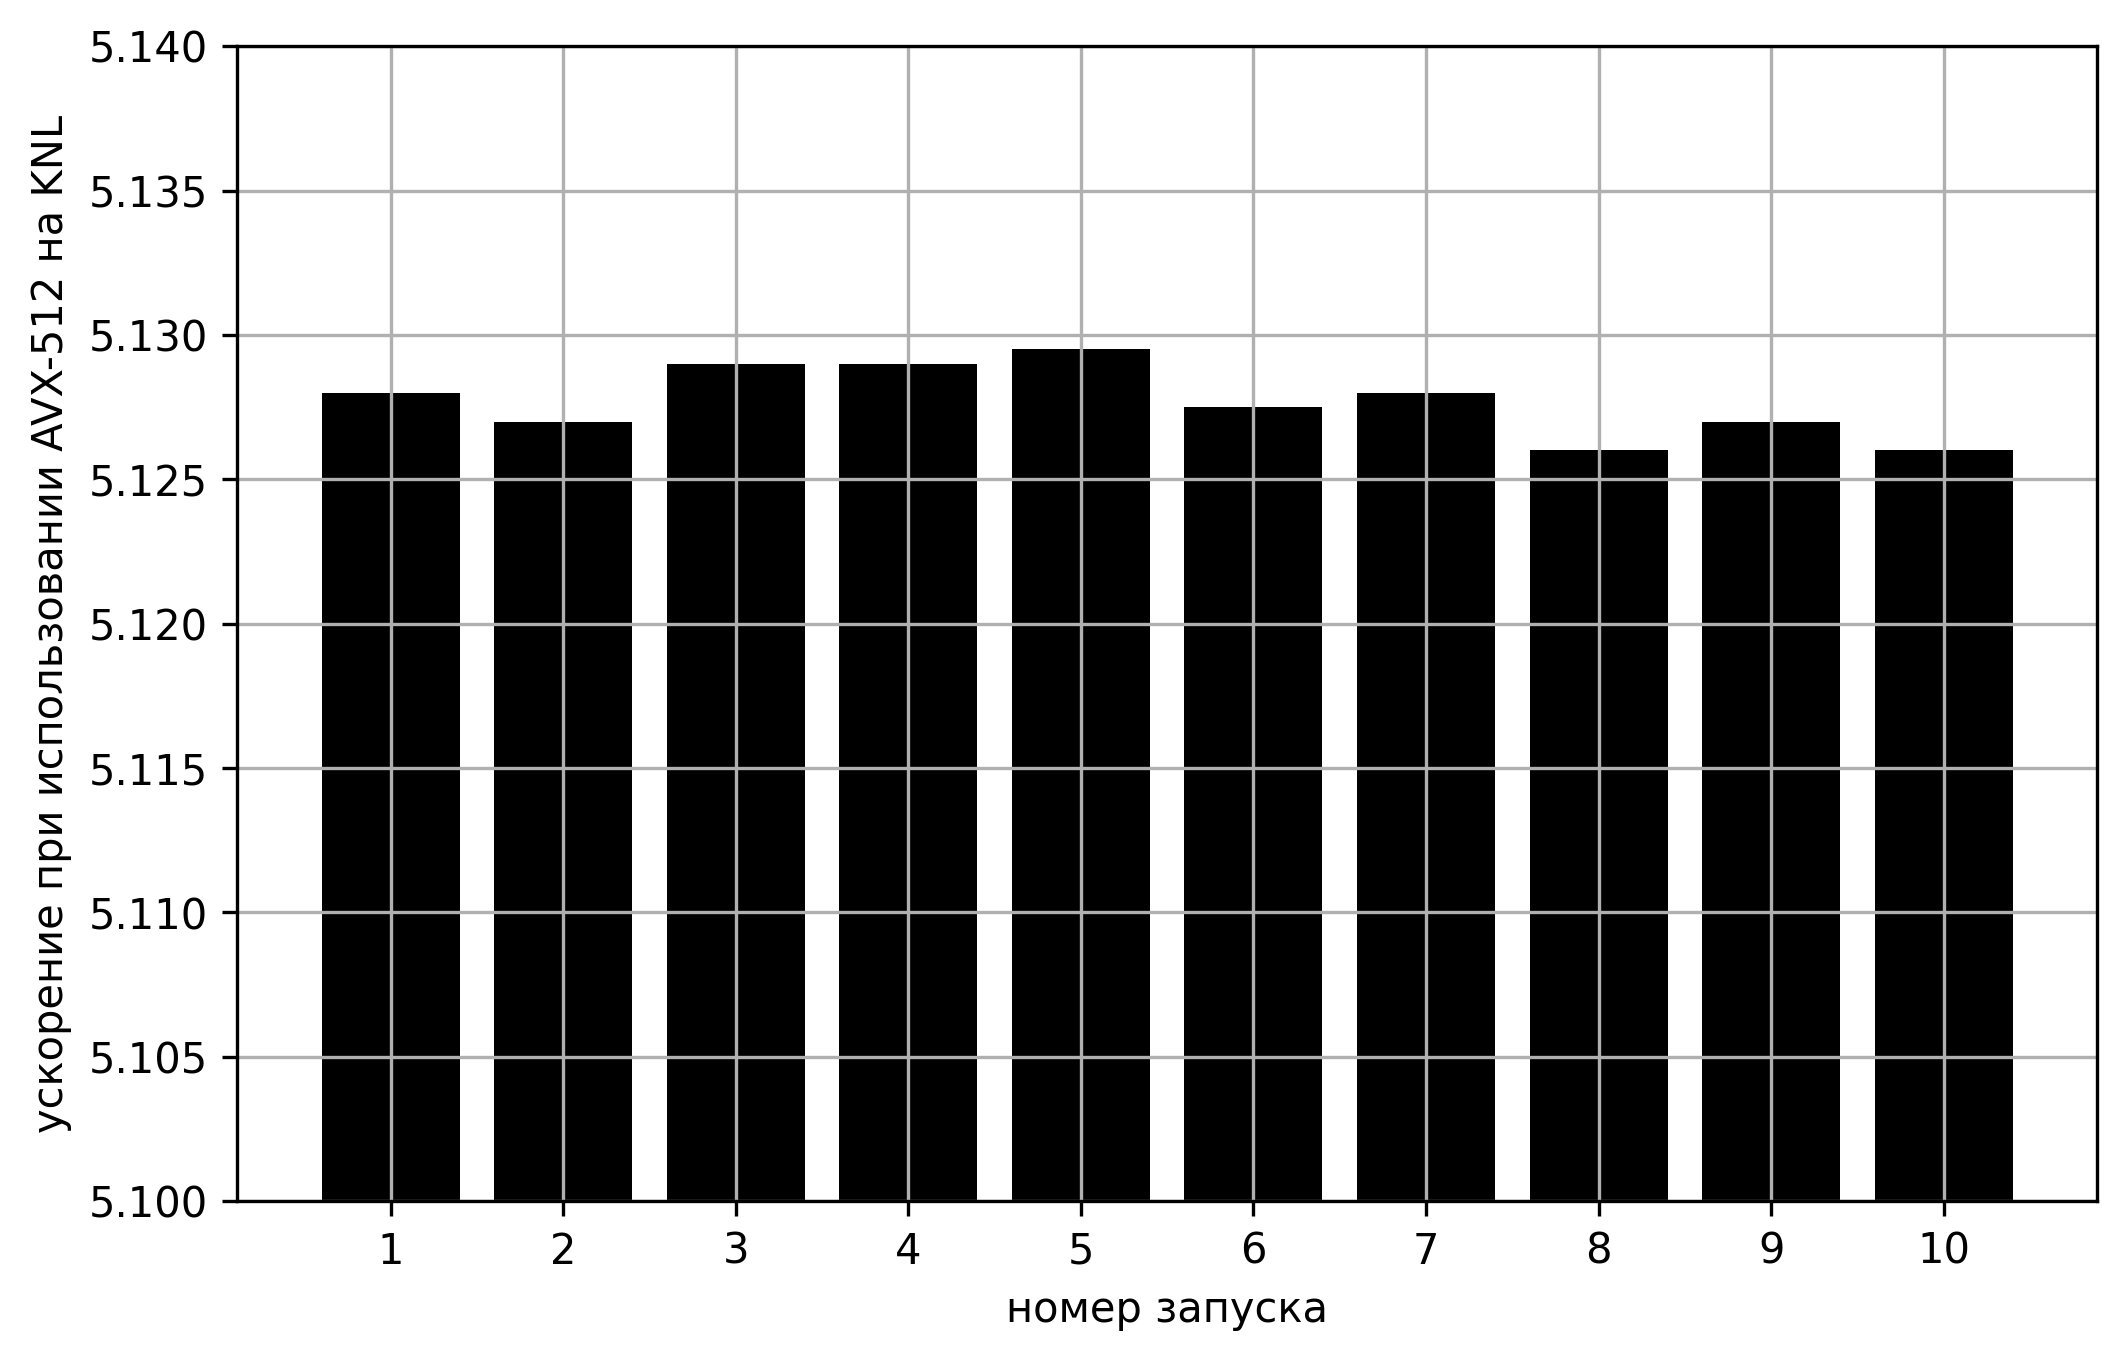
\includegraphics[width=0.8\textwidth]{./pics/text_4_vec_loc_branch/res.png}
	\caption{Ускорение от применения выноса маловероятного региона в задаче определения конфликта со спутными следами летательных аппаратов (для 10 запусков по $10^7$ окрестностей отрезков в каждом).}
	\label{fig:text_4_vec_loc_branch_res}
\end{figure}

\subsubsection{Выделение вероятного пути исполнения с помощью оптимизации <<черная дыра>>}

В этом разделе описан метод выноса маловероятных регионов из плоского цикла в общем случае с помощью подхода, который в некоторых источниках применительно к своим предметным областям встречается под названием blackhole (<<черная дыра>>) \cite{Ilbeyi2019}.

\begin{figure}[ht]
	\centering
	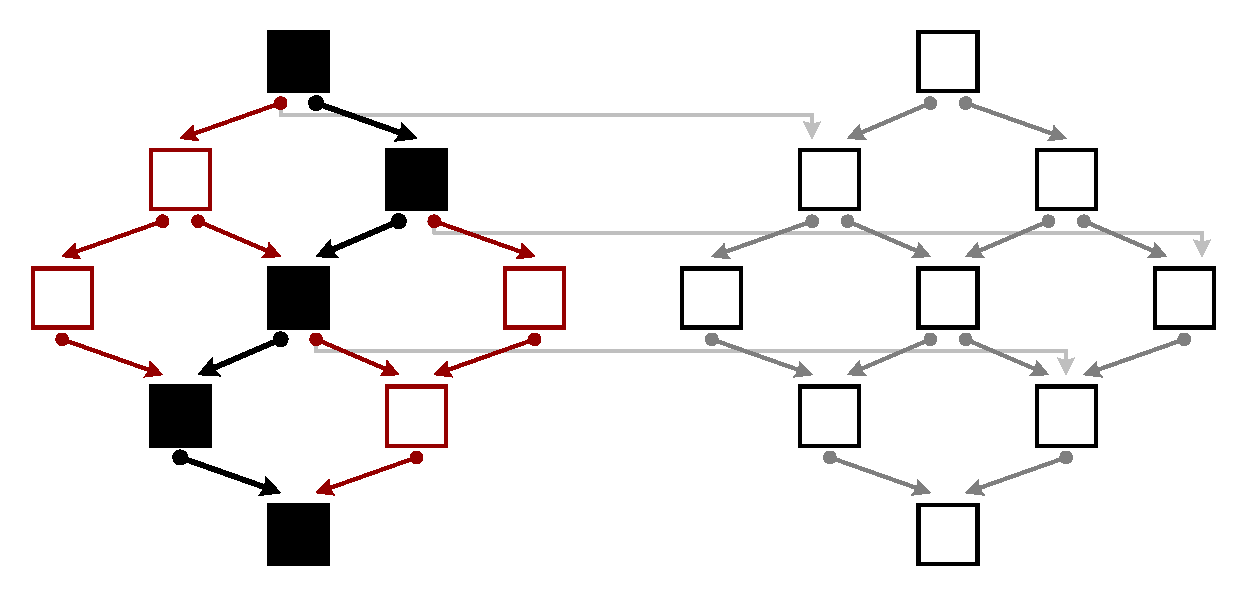
\includegraphics[width=1.0\textwidth]{./pics/text_4_vec_loc_branch/blackhole.pdf}
	\caption{Иллюстрация схемы работы оптимизации <<черная дыра>>.}
	\label{fig:text_4_vec_loc_branch_blackhole}
\end{figure}

Пусть дам некоторый CFG тела плоского цикла (рис.~\ref{fig:text_4_vec_loc_branch_blackhole} слева), в котором присутствует явно выделенный пусть исполнения (на рисунке выделен черным цветом), вероятность прохождения которого близка к единице \cite{Shabanov2021VecCFG}.
Другие крайне маловероятные линейные участки (выделенные на рисунке красным цветом) представляют собой программный контекст, который практически никогда не исполняется, и векторизацию которого проводить нецелесообразно, либо невозможно.
Оптимизация blackhole заключается в создании точной копии CFG, на которую перенаправляются все маловероятные переходы из основного тела.
После выполнения перенаправления маловероятных переходов все ребра и линейные участки, отмеченные на рис.~\ref{fig:text_4_vec_loc_branch_blackhole} красным цветом, могут быть удалены.
Таким образом, после выполнения оптимизации в качестве объекта векторизации остается ограниченный и пригодный к векторизации программный контекст.
В случае же если один из маловероятных переходов все же осуществится, то выполнится переход на точную копию изначального CFG, который хоть и не оптимально, но корректно отработает данную редкую ситуацию.
Эта оптимизация получила свое название blackhole потому что после выполнения редкого перехода на копию CFG программа не может вернуться обратно в векторизованную версию, в этом случае данный экземпляр плоского цикла закончит свое исполнение в <<черной дыре>>.
Оптимизация может применяться в различных вариациях.
Например, можно создавать копию не целого CFG, а только конкретных маловероятных регионов, в этом случае мы будем иметь оптимизацию локализации редких путей исполнения.
Наоборот, более консервативным вариантом оптимизации является перенаправление маловероятных переходов сразу на голову невекторизованной копии тела цикла, что соответствует просто проведению повторного расчета при возникновении исключительной ситуации.
